\section{Results}

For the initial~\SI{10}{\hertz} ramp function~(from zero to five volts), the
length of time devoted to each output voltage segment was measured with an
oscilloscope, as shown in Figure~\ref{f:time_step}.
%
\begin{figure}[H]
\centering
	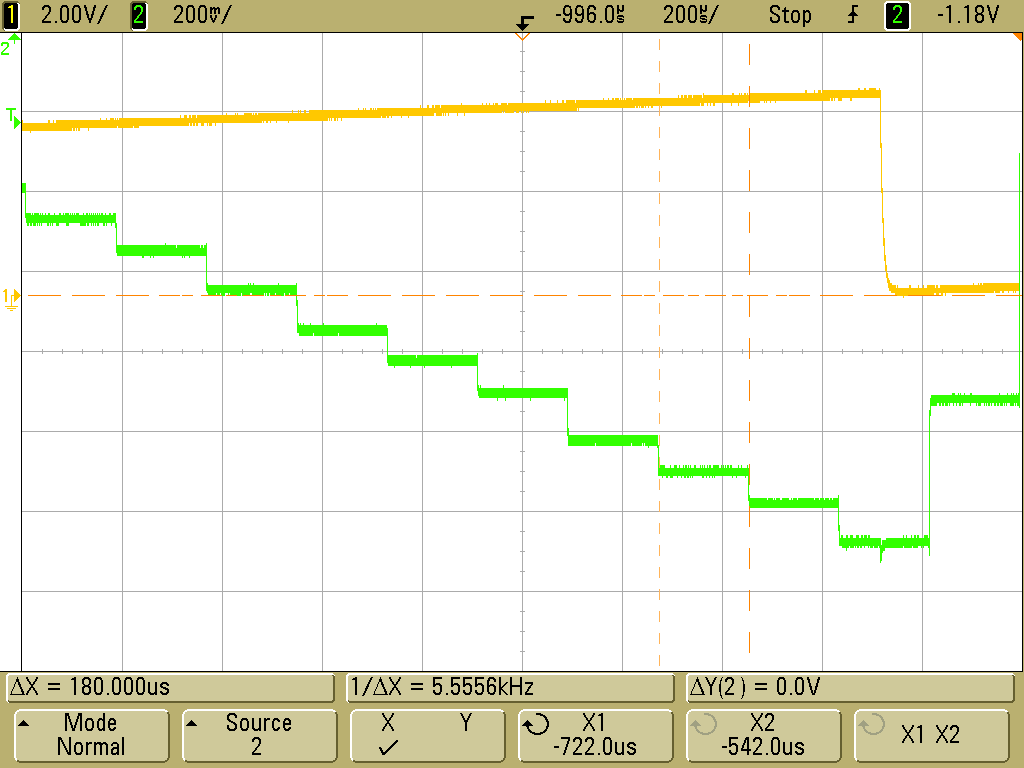
\includegraphics[width=.8\textwidth]{img/shot/ramp_timestep.png}
	\parbox{.8\textwidth}{
	\caption[Segment time]{Oscilloscope screenshot showing the width in time of
	one segment of the DAC output.}
	\label{f:time_step}}
\end{figure}
%
The oscilloscope measured the time step to be~\SI{180}{\micro\second}.  During
this span of time,
%
\begin{equation*}
	\SI{180}{\micro\second} \cdot \SI{379}{\kilo\hertz} = \SI{68.22}{cycles}
\end{equation*}
%
of the internal ADC clock pass (note that the clock frequency
of~\SI{379}{\kilo\hertz} was measured in step two).  This logically makes
sense, as it was observed in step two that each ADC measurement requires
roughly~70 clock cycles, and the ADC output is being directly fed into the
DAC's input in this step.

A similar test was performed with a sinusoidal signal of varying input
frequencies.  For very low frequency inputs, the output waveform closely mimicked
the input, as shown in Figure~\ref{f:100hz} for a~\SI{100}{\hertz} sine wave.
%
\begin{figure}[H]
\centering
	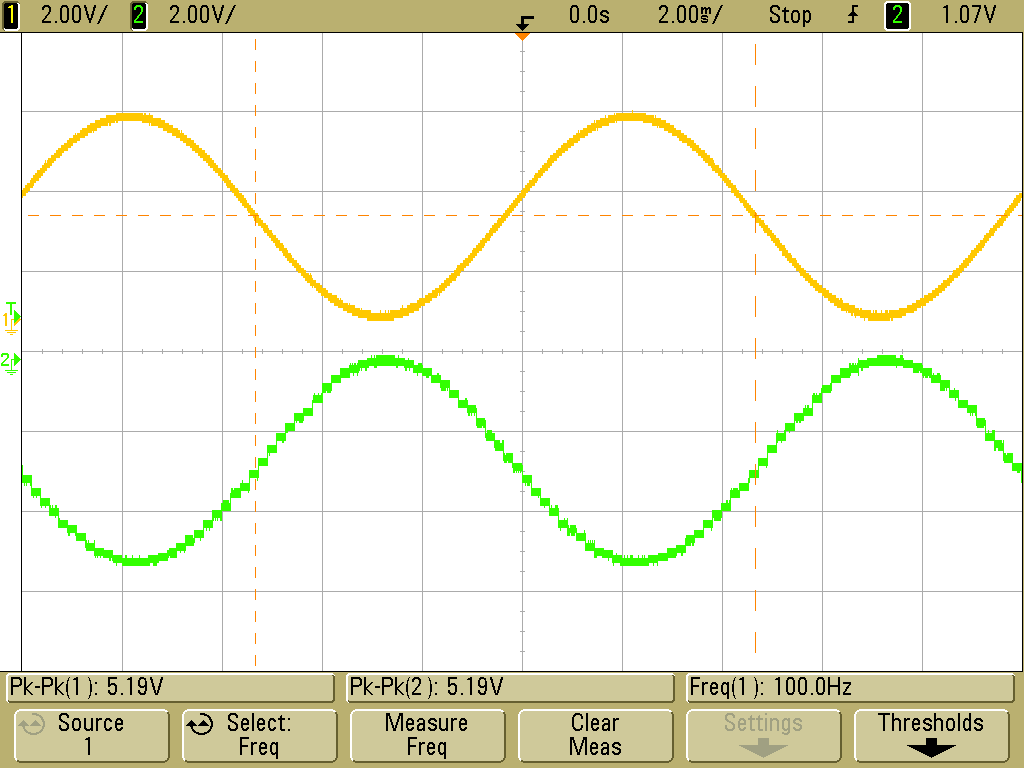
\includegraphics[width=.8\textwidth]{img/shot/sine_100hz.png}
	\parbox{.8\textwidth}{
	\caption[Sinusoidal input --- Low frequency]{Captured input~(upper) and output~(lower) of
	the ADC-DAC circuit.  Note the similarity between the two signals.}
	\label{f:100hz}}
\end{figure}

For high-frequency sinusoidal inputs, the system failed to accurately recreate
the input signal.  For the case of the built circuit, this failure occurred
at~\SI{3000}{\hertz}, shown in Figure~\ref{f:3000hz}.
%
\begin{figure}[H]
\centering
	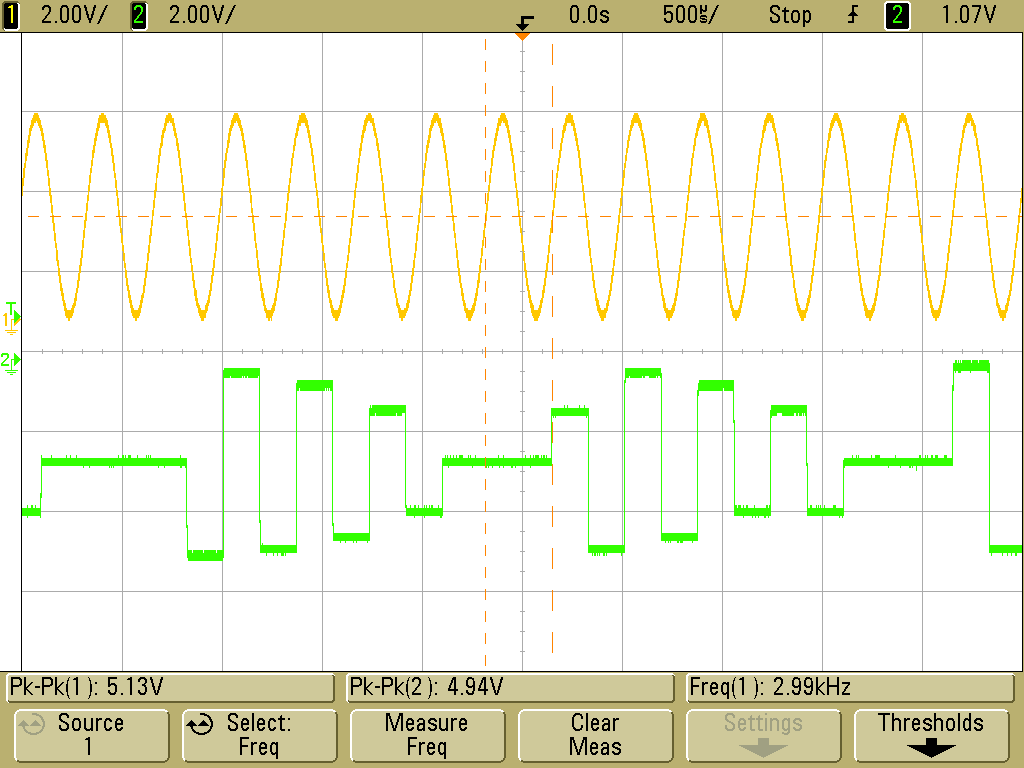
\includegraphics[width=.8\textwidth]{img/shot/sine_3000hz.png}
	\parbox{.8\textwidth}{
	\caption[Sinusoidal input --- Failure]{Failed recreation of the input
	signal by the combined ADC-DAC system.  This oscilloscope screenshot was
	captured for a sinusoidal input of~\SI{3}{\kilo\hertz}.}
	\label{f:3000hz}}
\end{figure}
%
A sinusoid of~\SI{3000}{\hertz} has a period of
just~$0.33\overline{3}\si{\micro\second}$ --- a period that is an order of
magnitude below the~\SI{2.639}{\micro\second} period of the internal ADC clock.
A signal with such a small period is impossible to represent with such a slow
clock frequency, and results in the aliasing shown in Figure~\ref{f:3000hz}.
